%
% Preable
%

\documentclass{amsart}

%
%  packages
%

\usepackage{amsfonts, amsthm, amssymb, amsmath, stmaryrd, etoolbox}
\usepackage{comment}
\usepackage{mathtools}
\usepackage{graphicx,caption,subcaption}
\usepackage{todonotes}
\usepackage{xcolor}
\usepackage{url}
\usepackage{subfiles}
%\usepackage[backend=bibtex,citestyle=numeric]{biblatex}
\usepackage[inline]{enumitem}
	\setlist{itemsep=0em, topsep=0em, parsep=0em}
	\setlist[enumerate]{label=(\alph*)}
\usepackage[breaklinks=true]{hyperref}
	\definecolor{hyperrefcolor}{rgb}{0,0,0.7}
	\hypersetup{colorlinks,linkcolor={hyperrefcolor},citecolor={hyperrefcolor},urlcolor={hyperrefcolor}}
\usepackage{tikz}
\usepackage[all,2cell]{xy}
	\usetikzlibrary{matrix,arrows,shapes,decorations.markings,decorations.pathreplacing}

%
% commands
%

\newcommand{\RR}{\mathbb{R}}
\newcommand{\ZZ}{\mathbb{Z}}
\newcommand{\NN}{\mathbb{N}}
\newcommand{\QQ}{\mathbb{Q}}
\newcommand{\CC}{\mathbb{C}}
\newcommand{\DD}{\mathbb{D}}
\newcommand{\MM}{\mathbb{M}}
\renewcommand{\epsilon}{\varepsilon}

\newcommand{\op}[1]{\operatorname{#1}}
\newcommand{\cat}[1]{\mathbf{#1}}
\newcommand{\dblcat}[1]{\mathbb{#1}}
\renewcommand{\t}[1]{\text{#1}}

\newcommand{\from}{\colon}
\newcommand{\xto}[1]{\xrightarrow{#1}}
\newcommand{\sm}{\smallsetminus}
\newcommand{\tospan}{\xrightarrow{\mathit{sp}}}
\newcommand{\tocospan}{\xrightarrow{\mathit{csp}}}
\newcommand{\diagram}[1]{\raisebox{-0.5\height}{\includegraphics{#1}}}

\newcommand{\bispmap}[1]{\mathbf{Sp(#1)}}
\newcommand{\dblspmap}[1]{\mathbb{S}\mathbf{p(#1)}}
\newcommand{\bicspmap}[1]{\mathbf{Csp(#1)}}
\newcommand{\dblcspmap}[1]{\mathbb{C}\mathbf{sp(#1)}}
\newcommand{\bispsp}[1]{\mathbf{Sp(Sp(#1))}}
\newcommand{\dblspsp}[1]{\mathbb{S}\mathbf{p(Sp(#1))}}
\newcommand{\bicspcsp}[1]{\mathbf{Csp(Csp(#1))}}
\newcommand{\dblcspcsp}[1]{\mathbb{C}\mathbf{sp(Csp(#1))}}
\newcommand{\bimonspcsp}[1]{\mathbf{MonicSp(Csp(#1))}}
\newcommand{\dblmonspcsp}[1]{\mathbb{M}\mathbf{onicSp(Csp(#1))}}
\newcommand{\biepiccspsp}[1]{\mathbf{EpicCsp(Sp(#1))}}
\newcommand{\dblepiccspsp}[1]{\mathbb{E}\mathbf{picCsp(Sp(#1))}}
\newcommand{\spcsp}[1]{\mathbf{Sp(Csp(#1))}}
\newcommand{\dblspcsp}[1]{\mathbb{S}\mathbf{p(Csp(#1))}}

%
% math operators
%

\DeclareMathOperator{\Hom}{Hom}
\DeclareMathOperator{\id}{id}
\DeclareMathOperator{\ob}{Ob}
\DeclareMathOperator{\arr}{arr}
\DeclareMathOperator{\im}{im}
\DeclareMathOperator{\Aut}{Aut}
\DeclareMathOperator{\Bij}{Bij}
\DeclareMathOperator{\Sub}{Sub}
\DeclareMathOperator{\colim}{colim}

%
% envirnments and counters
%

\newtheorem{thm}{Theorem}[section]
\newtheorem{lem}[thm]{Lemma}
\newtheorem{prop}[thm]{Proposition}
\newtheorem{cor}[thm]{Corollary}

\theoremstyle{remark}
	\newtheorem{remark}[thm]{Remark}
	\newtheorem{notation}[thm]{Notation}

\theoremstyle{definition}
	\newtheorem{ex}[thm]{Example} 
	\newtheorem{defn}[thm]{Definition}

% \setcounter{tocdepth}{1} % Sets depth for table of contents. 

%
% tikz types
%

\tikzset{rewritenode/.style={shape=circle,fill=rewritecolor,scale=0.25,font=\Huge}}
\tikzset{RWopen/.style={shape=circle,draw=black,fill=white,scale=0.5,font=\Huge}}
\tikzset{RWclosed/.style={shape=circle,fill=black,scale=0.5,font=\Huge}}
\tikzset{CDnode/.style={shape=circle,fill=white,scale=.5}}
\tikzset{zxgreen/.style={shape=circle,draw,thick,fill=green}}
\tikzset{zxred/.style={shape=circle,draw,thick,fill=red}}
\tikzset{zxyellow/.style={shape=rectangle,draw,thick,fill=yellow}}
\tikzset{zxdiamond/.style={shape=diamond,fill=black,inner sep=2.75}}
\tikzset{zxopen/.style={shape=circle,draw,thick,inner sep=2pt}}
\tikzset{->-/.style={decoration={%
			markings,
			mark=at position .5 with {\arrow{>}}},postaction={decorate}}
}
\tikzset{->-pos/.style={decoration={%
			markings,
			mark=at position #1 with {\arrow{>}}},postaction={decorate}}
}
\tikzset{->-/.style={decoration={%
			markings,
			mark=at position .5 with {\arrow{>}}},postaction={decorate}}
}
\tikzset{->-pos/.style={decoration={%
			markings,
			mark=at position #1 with {\arrow{>}}},postaction={decorate}}
}

%
% defining arrow with a vertical line through it
%

\makeatletter
\def\slashedarrowfill@#1#2#3#4#5{%
	$\m@th\thickmuskip0mu\medmuskip\thickmuskip\thinmuskip\thickmuskip
	\relax#5#1\mkern-7mu%
	\cleaders\hbox{$#5\mkern-2mu#2\mkern-2mu$}\hfill
	\mathclap{#3}\mathclap{#2}%
	\cleaders\hbox{$#5\mkern-2mu#2\mkern-2mu$}\hfill
	\mkern-7mu#4$%
}
\def\rightslashedarrowfill@{%
	\slashedarrowfill@\relbar\relbar\mapstochar\rightarrow}
\newcommand{\xslashedrightarrow}[2][]{%
	\ext@arrow 0055{\rightslashedarrowfill@}{#1}{#2}}
\makeatother

\newcommand{\hto}{\xslashedrightarrow{}}

%
% bibliography  
% \addbibresource{Catfying_zxCalc--Bibliography.bib}





\begin{document}
	


\begin{ex}
	A \emph{corelation} between objects $X$ and $Y$ of a category is a co-subobject of $X+Y$, or rather an equivalence class of epimorphisms $X+Y \to C$ for some object $C$. Taking finite sets and corelations between them gives a symmetric monoidal category $\cat{Corel}$.  Set theoretically, a corelation $C \from X \nrightarrow Y$  is simply an equivalence relation on $X+Y$ given by taking the fibers of the surjection $X+Y \to C$. We get an category $\bispmap{FinSet}_{\text{JE}}$ equivalent to $\cat{Corel}$ by taking the subcategory of finite sets and cospans consisting of all objects and jointly epic cospans.  We can promote $\bispmap{FinSet}_{\text{JE}}$ to a bicategory by defining $\bispmap{FinSet}_{\text{JE}}(X,Y)$ to consist of all maps of cospans. Hence $\bispmap{FinSet}_{\text{JE}}(X,Y)$ is equivalent to the full subcategory of the over-category $X+Y/\cat{FinSet}$ whose objects are the surjective maps $X+Y \to C$. So a $2$-morphism in $\bispmap{FinSet}_{\text{JE}}$ is really just a commuting diagram
	\[
	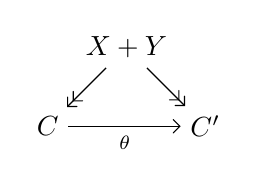
\begin{tikzpicture}
		\node (A) at (0,1) {$X+Y$};
		\node (B) at (-1,0) {$C$};
		\node (C) at (1,0) {$C'$};
		%
		\path[->,font=\scriptsize,>=angle 90]
		(A) edge[->>] node[above]{$$} (B)
		(A) edge[->>] node[above]{$$} (C)
		(B) edge node[below]{$\theta$} (C);
	\end{tikzpicture}
	\]
	Note that $\bispmap{FinSet}_{\text{JE}}(X,Y)$ is locally posetal -- that is if $\theta$ does exist, it is the unique $2$-morphism $C \Rightarrow C'$.  Indeed, for $c \in C$, the fiber of $c$ is contained in the fiber of $\theta (c)$ meaning that $\theta$ is completely determined by the corelations.  Inspiration now leads us to promote $\cat{Corel}$ to a bicategory by inserting a $2$-morphism
	\[
	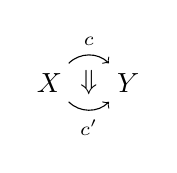
\begin{tikzpicture}
		\node (X) at (0,0) {$X$};
		\node (Y) at (1,0) {$Y$};
		%
		\path[->,font=\scriptsize]
		(X) edge[out=45,in=135] node[above]{$c$} (Y)
		(X) edge[out=-45,in=-135] node[below]{$c'$} (Y);
		%
		\node () at (0.5,0) {$\Downarrow$};
	\end{tikzpicture}
	\]
	whenever the equivalence relation given by $c$ is contained in that given by $c'$. There is an obvious biequivalence between $\cat{Corel}$ and $\bispmap{FinSet}_{\text{JE}}$. Hence $\cat{Corel}$ is a bicategory of cospans.
\end{ex}

% EXAMPLE: LIN REL
%
\begin{ex}
	The category $\cat{LinRel}$ of finite dimensional vector spaces and linear relations (subspaces of $V \oplus W$) plays an important role in network theory \cite{BaezErbele_CatControl,FongSobocRap}. As in Fong's thesis \cite{Fong_Thesis},
	we can identify $\cat{LinRel}$ with the subcategory of the category $\bispmap{FinVec}$ containing all finite dimensional vector spaces and jointly monic spans. The idea is that a jointly monic span $L \from V \tospan W$ gives an injection $L \to V \oplus W$, hence a linear relation $L \from V \nrightarrow W$. Consider the full sub-bicategory $\bispmap{FinVec}_{\text{JM}}$ of $\bispmap{FinVec}$ with all finite dimensional vector spaces and jointly monic spans. Similar to the previous example, the category $\bispmap{FinVec}_{\text{JM}}(V,W)$ is equivalent to the full subcategory of the over-category $\bispmap{FinVec}_{\text{JM}}/V \oplus W$ consisting of monics $L \to V \oplus W$.  Thus, a $2$-morphism can be thought of as the diagram
	\[
	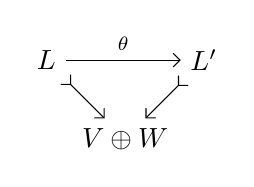
\begin{tikzpicture}
		\node (A) at (0,0) {$V \oplus W$};
		\node (B) at (-1,1) {$L$};
		\node (C) at (1,1) {$L'$};
		%
		\path[->,font=\scriptsize,>=angle 90]
		(B) edge[>->] node[above]{} (A)
		(C) edge[>->] node[above]{} (A)
		(B) edge node[above]{$\theta$} (C);
	\end{tikzpicture}
	\]
	It is easy to see that $\theta$ is monic and is the unique such morphism making these diagrams commute, assuming that it exists. As above, we promote $\cat{LinRel}$ to a bicategory by introducing a $2$-morphism 
	\[
	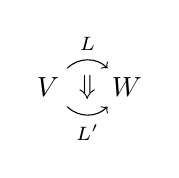
\begin{tikzpicture}
		\node (V) at (0,0) {$V$};
		\node (W) at (1,0) {$W$};
		%
		\path[->,font=\scriptsize]
		(V) edge[out=45,in=135] node[above]{$L$} (W)
		(V) edge[out=-45,in=-135] node[below]{$L'$} (W);
		%
		\node () at (0.5,0) {$\Downarrow$};
	\end{tikzpicture}
	\]
	whenever $L \subseteq L'$.  Hence, $\cat{LinRel}$ is a bicategory of spans.
\end{ex}



\end{document}